%%%%%%%%%%%%%%%%%%%%%%%%%%%%%%%%%%%%%%%%%
% Avi's Project Proposal
%
% Summer Research Project 
%
%%%%%%%%%%%%%%%%%%%%%%%%%%%%%%%%%%%%%%%%%

%----------------------------------------------------------------------------------------
%	PACKAGES AND DOCUMENT CONFIGURATIONS
%----------------------------------------------------------------------------------------

\documentclass{article}

\usepackage[version=3]{mhchem} % Package for chemical equation typesetting
\usepackage{siunitx} % Provides the \SI{}{} and \si{} command for typesetting SI units
\usepackage{graphicx} % Required for the inclusion of images
\usepackage{natbib} % Required to change bibliography style to APA
\usepackage{amsmath} % Required for some math elements 
\usepackage{gensymb}

\setlength\parindent{0pt} % Removes all indentation from paragraphs

\renewcommand{\labelenumi}{\alph{enumi}.} % Make numbering in the enumerate environment by letter rather than number (e.g. section 6)

%\usepackage{times} % Uncomment to use the Times New Roman font


%Code packages
\usepackage{indentfirst}
\usepackage[utf8]{inputenc}
\usepackage{listings}
\usepackage{color}
% Code packages end


%----------------------------------------------------------------------------------------
%	DOCUMENT INFORMATION
%----------------------------------------------------------------------------------------

\title{Project Plan} % Title
			 
\author{Avi \textsc{Vajpeyi}} % Author name

\date{\today} % Date for the report

\begin{document}

\maketitle % Insert the title, author and date


%have an understanding of what you will do and why the work is necessary or desirable
%It outlines the approach you will take to carry out your task
%It provides a schedule or timeline for accomplishing the individual steps and overall goals of your project
%It encourages your mentor and his or her staff to make the arrangements necessary to accommodate you and your needs before your arrival




 \begin{abstract}
On September 14th, 2015, the Advanced LIGO detected the first gravitational wave \cite{DetectionPaper}. The detected wave had a very large Signal to Noise Ratio value, which made it stand out from the rest of the candidate events. This paper investigates an alternative detection statistic, involving the `Bayes Factor.' This detection statistic might prove to be more robust than SNR, as it may be able better to discern between strains due to gravitational waves, and strains due to noise. This study of the new detection statistic is focused on binary black hole systems. 


\end{abstract}

%----------------------------------------------------------------------------------------
%	SECTION 1
%----------------------------------------------------------------------------------------

\section{Introduction}




 \indent The completion of the two Advanced Laser Interferometer Gravitational-Wave Observatories has led to the discovery of a gravitational-wave signal \cite{DetectionPaper}. This paper deals with a new detection statistic, involving Bayesian statistics, to rank the different candidate events (the strains in the data sets that could potentially be due to gravitational waves). The candidate events we focus on are from binary black hole systems as they are believed to be fairly common in the Universe \cite{NumDetections}. Before we study this new method, we will discuss how data is currently being recorded and analysed.\\
 
 
 
 
 % How Ligo detects signals
 \indent Each of the advanced LIGO observatories uses a modified Michaelson Interferometer that measures the difference in the length of the orthogonal arms of the observatory to detect the presence of a gravitational wave \cite{DetectionPaper}. On passing, a gravitational wave alters the difference between the arm lengths, which helps determine the gravitational-wave strain amplitude. \\
  
  
  
  % how signal is found in data
  \indent To determine if data recorded by LIGO stores gravitational wave information, the data is processed with two search techniques. One search looks for generic transient waveforms (unmodeled or unexpected waveforms) in data \cite{Enia}. The second is a match filtered search that compares the data with templates of waveforms generated by general relativity \cite{Enia}.\\
  
  
  % Discussion on how background noise is removed with time shifts, and how data is ranked 
  \indent Both the search processes are made challenging due to the background noise present in the data. The background noise can result with strains in the data similar to strains from gravitational waves \cite{DetectionPaper}. This background noise can result from defects in a mirror, the uncertainty in the number of photons traveling in a the laser beam (shot noise), seismic activity, or even thermal noise generated by the Brownian motion of electrons inside circuits \cite{RSmith}. To separate  strains caused by background noise from those caused by gravitational waves, the data from one LIGO observatory is compared with another LIGO observatory's data \cite{DetectionPaper}. To compare the data sets, one of the them can be time-shifted so that it matches the data in the other detector over the light-travel time between the detectors. That is, one data set can be time-shifted so that both of the data sets lie along the same interval of time.\\
  
  After making the necessary time shift, events present in one data set but not the other become apparent. If a strain is not present in both data sets, the strain may have resulted from noise in one of the detectors, as a gravitational wave strain would be observed in both detectors \cite{DetectionPaper}. Hence, all the strains that cannot be correlated with a data set taken from another observatory are discounted as strains due to noise \cite{DetectionPaper}. This process cuts a majority of the strains that may have been present due to noise\cite{DetectionPaper}. We attempt to discount any remaining noise-strains by implementing a detection statistic to rank the strains according to the likelihood that the strain resulted from a gravitational wave.\\
  
    % Talk about Time-frequency morphology classes, and how certain classes can be discounted? That is more specific to Generic...
  
  % SNR as a detection statistic 
  \indent The detection statistic currently being used to rank strains according to the maximum likelihood of it being due to a gravitational wave is the signal-to-noise ratio (SNR) detection technique \cite{Enia}. This method compares the power of the strain signal to the power of the remaining noise at a given point \cite{RSmith}. Although the power of the noise is difficult to calculate, we know that this ranking process can make some gravitational wave strains stand out, as seen from the Fig~\ref{Fig:Detection}.  However, we believe that this method lacks the sensitivity necessary to detect some gravitational waves that do not have SNR values as high as those of GW150914. Hence we would like to investigate an alternate detection statistic, specifically one that compares the relative probability that a data set contains a strain due to a gravity wave to the probability that the data just contains noise. This ratio is known as the Bayes Factor. %Additionally, it is believed that this detection statistic might help increase the detection rate of gravitational waves by a factor of 10, as  [Not sure what to cite here - could not find mention of this in Enia's paper]. 
  
\begin{figure}[h]
	\caption{Search results of the generic transit search in which the first gravitational wave signal, marked GW150914, was detected. The wave strain of GW150914 stands out as the strongest strain in the entire search. Figure taken from \cite{DetectionPaper}}
	\centering
	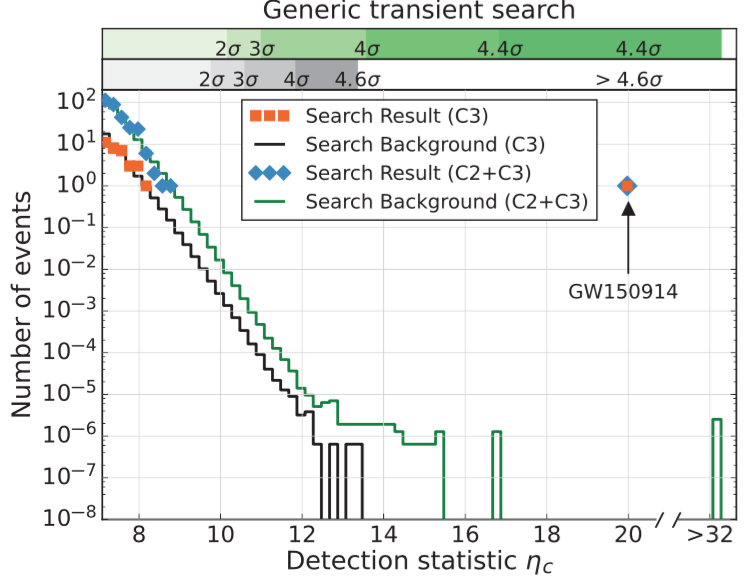
\includegraphics[width=0.5\textwidth]{DetectionInGenericTransientSearch} \label{Fig:Detection}
\end{figure}

 
 %----------------------------------------------------------------------------------------
 %	SECTION 2
 %----------------------------------------------------------------------------------------
 
 
 \section{Objectives}
 
 We have seen that using SNR for detection has been successful, as the gravitational wave GW150914 was detected with it \cite{DetectionPaper}. However, we would like to investigate a more robust detection statistic using the Bayes Factor and focus our search to binary black hole systems. This detection statistic would involve comparing the probability that the signal data contains a strain due to gravitational waves to the probability that the signal does not contain a strain due to a gravitational wave. \\
 
 
 
 To calculate Bayes' Factor, we first need to determine the posterior probability density function (PDF). For gravitational wave analysis, the PDF of the parameters $\vec{\theta}$ is \cite{RSmith}:
 
 %equation of bayes factor\\
\begin{equation} \label{eq:bayesTheorem}
p(\vec{\theta}|d, \mathcal{H})  = \frac{p(\vec{\theta}| \mathcal{H}) \ p(d|\vec{\theta},  \mathcal{H}) }  { p(d|\mathcal{H})},
\end{equation} 
 
 or in other terms, 
 
 \begin{equation} \label{eq:englishTheorem}
{ Posterior \ Probability \ Density \ Function}  = \frac{ Likelihood  \times Prior}{Evidence}. \nonumber
 \end{equation} 
 
 In this equation, we have each model $ \mathcal{H}_i$, to have a vector of parameters $\vec{\theta}$, with which we can calculate a `Prior' distribution of $P(\vec{\theta}| \mathcal{H})$. This states what values the model $ \mathcal{H}_i$ might be expected to take from the data set $d$. We also have $p(d|\vec{\theta},  \mathcal{H})$, which is the `likelihood' of the data, given that the model $ \mathcal{H}_i$ is true. Additionally, we have $p(d|\mathcal{H})$ which is the `evidence,' according to \cite{BaeStats}.\\
 
We can compare two models, $ \mathcal{H}_a$ and  $ \mathcal{H}_b$ by calculating the relative probabilities as 
 \begin{align} \label{eq:englishTheorem}
 Relative \ Probabilities &= \frac{p(\vec{\theta}| \mathcal{H}_a) }{p(\vec{\theta}| \mathcal{H}_b)} \frac{p(d|\vec{\theta},  \mathcal{H}_a)}{p(d|\vec{\theta},  \mathcal{H}_b)}\nonumber\\
 &= B_{ab} \frac{p(\vec{\theta}| \mathcal{H}_a) }{p(\vec{\theta}| \mathcal{H}_b)}, \nonumber
 \end{align} 
where $B_{ab}$ is the `Bayes' Factor,' which is equal to \cite{BaeStats}:\\
\begin{equation}
B_{ab} = \frac{p(\vec{\theta}| \mathcal{H}_a) }{p(\vec{\theta}| \mathcal{H}_b)}.
 \end{equation}
 
 Using the Bayes' Factor, we may be able to better highlight the strains due to gravitational waves against strains due to noise. This could raise the number of detections of gravitational waves generated by binary black hole systems. With more detections, we could have more data on the masses and spins of black holes in our Universe. With these results, we would be able to gain an estimate of the population of black holes in our Universe. [Not sure what to cite here - I got this from the project abstract]
 %----------------------------------------------------------------------------------------
 %	SECTION 3
 %----------------------------------------------------------------------------------------
 
 
 \section{Approach}
 The main objective of this project will be to asses the sensitivity of the Bayes' Factor to rank gravitational waves that might have been missed using SNR as the detection-statistic. After writing a procedure using the Bayes' Factor to rank various events, we will create a distribution of the background noise with this new detection statistic. This will be done by injecting gravity wave strains into data sets containing noise. Once we have calculated the search background, we will be able to compute the Bayes' Factor for several quiet events that appeared on the background of SNR, as seen in Fig~\ref{Fig:Detection}.
 
 
 
 %----------------------------------------------------------------------------------------
 %	SECTION 4
 %----------------------------------------------------------------------------------------
 
 
 \section{Project Schedule}
 
 %----------------------------------------------------------------------------------------
 %	REFERENCES
 %----------------------------------------------------------------------------------------
 
---------------------------------------------------------------------
 
 \bibliographystyle{plain}		% Using this bibliography style will ignore the annotations.
 
 \bibliography{ProjectProposalRefrences}
 
%----------------------------------------------------------------------------------------


\end{document}